\documentclass{article}
\usepackage[dvips]{graphicx}
\usepackage{float}
\usepackage{graphics} 
\usepackage{graphicx}
\usepackage{color}
\usepackage{subfig}
%\usepackage[subnum]{cases}
\usepackage{amsmath}
\usepackage{amsthm}
\usepackage{amsfonts}
\usepackage{pifont}
\usepackage{rotating}
\usepackage{latexsym}
\usepackage{verbatim}
%\usepackage[latin1]{inputenc}
\usepackage{multirow}
\usepackage{afterpage}
\usepackage{epsfig}
\usepackage{lscape}
\usepackage{makeidx}
\usepackage{tikz}
\usepackage{todonotes}
\usetikzlibrary{shapes,arrows,positioning,backgrounds,calc,petri,calc,fit}
%\tikzstyle{comp} = [draw, fill=blue!20, rectangle, minimum height=7mm, minimum width=14mm]
\tikzstyle{comp} = [draw, rectangle, minimum height=7mm, minimum width=14mm]
%\tikzstyle{voter} = [draw, fill=blue!20, circle, minimum height=7mm, minimum width=7mm]
\tikzstyle{voter} = [draw, circle, minimum height=7mm, minimum width=7mm]
%\tikzstyle{ftreeevent} = [draw, fill=blue!20, ellipse, minimum height=7mm, minimum width=14mm]
\tikzstyle{ftreeevent} = [draw, ellipse, minimum height=7mm, minimum width=14mm]
%\tikzstyle{state} = [draw, fill=blue!20, circle, minimum height=7mm, minimum width=7mm]
\tikzstyle{state} = [draw, circle, minimum height=7mm, minimum width=7mm]
%\tikzstyle{statebig} = [draw, fill=blue!20, circle, minimum height=11mm, minimum width=11mm]
\tikzstyle{statebig} = [draw, circle, minimum height=11mm, minimum width=11mm]
%[state/.style={circle,draw,thick,minimum size=5mm, node distance=2cm and 2cm}]

\tikzset{imtransition/.style={rectangle,draw=black,fill=black,thick,inner sep=0pt,minimum height=5mm,minimum width=0.05mm}}
\tikzset{every place/.style={minimum size=5mm,thick}}
\tikzset{every transition/.style={thick,draw=black,fill=black,minimum height=5mm,minimum width=0.5mm}}
%\tikzset{transitionr/.style={rectangle,thick,draw=black,fill=black,minimum width=5mm,minimum height=0.05mm}}
\tikzset{transitionr/.style={rectangle,draw=black,fill=black,thick,inner sep=0pt,minimum height=1mm,minimum width=5mm}}
\tikzset{every label/.style= black}
\graphicspath{{./fig/}}
%
\title{Dependability Analysis of Two Candidate\\ Architectures for a Brake-By-Wire System \\
\vspace{2.0cm}
\small Laboratory report in \\ EDA122 Fault-Tolerant Computer Systems \\[5ex]} % Title
\vspace{2.0cm}
\vfill
\author{Insert your name\\ Insert your name\\ \small Group\\
\vspace{5.0cm}
\\ \small Chalmers University of Technology \\
\small Gothenburg, Sweden 2012\\
\small Version no.: 0.0\\
} % Author name


\begin{document}

\maketitle % Insert the title, author and date
%
%\setlength\parindent{0pt} % Removes all indentation from paragraphs
%
%\renewcommand{\labelenumi}{\alph{enumi}.} % Make numbering in the enumerate environment by letter rather than number (e.g. section 6)
\newpage
\tableofcontents

\newpage
\section{Introduction}
\label{S1}
The purpose of this laboratory assignment is to gain understanding about how dependability modeling can be applied to evaluate fault-tolerant systems. In this report, two different design solutions for a brake-by-wire systems is evaluated.
 
In a brake-by-wire system, the conventional hydraulic is replaced by an electronic system. The advantage to use a electronic system instead of the conventional is lower weight, lower cost, and simpler integration with other electronic systems already in use, such as active safety systems and stability control. 


The model used for a brake-by-wire system is shown in \figref{bbwsys} and comprises of a central unit (CU) that receives sensor data about the car's movement and anticipated movement, four wheel units (WU) that measures and controls the rotation of a wheel, and serial buses (SB1 and SB2) for communication. To ensure fault tolerant behavior, the CU and WU are implemented using redundant components when found necessary, and the communication buses are duplicated. 

Individual brake commands is derived for the wheels with respect to the received sensor data and these computations can either be performed in the CU or in the WUs. The first architecture is called the distributed architecture, where the computations are performed in the WUs. The second architecture is called the centralized architecture, where the computations are performed in the CU.

The report are organized as follows. In \secref{S2}, the two design solutions are presented. In \secref{S3} is the dependability models used in the report explained. In \secref{S4} are the results presented. In \secref{S5}, the results are discussed and the report is conluded in \secref{S6}.

\begin{figure}[h!]
  \centering
  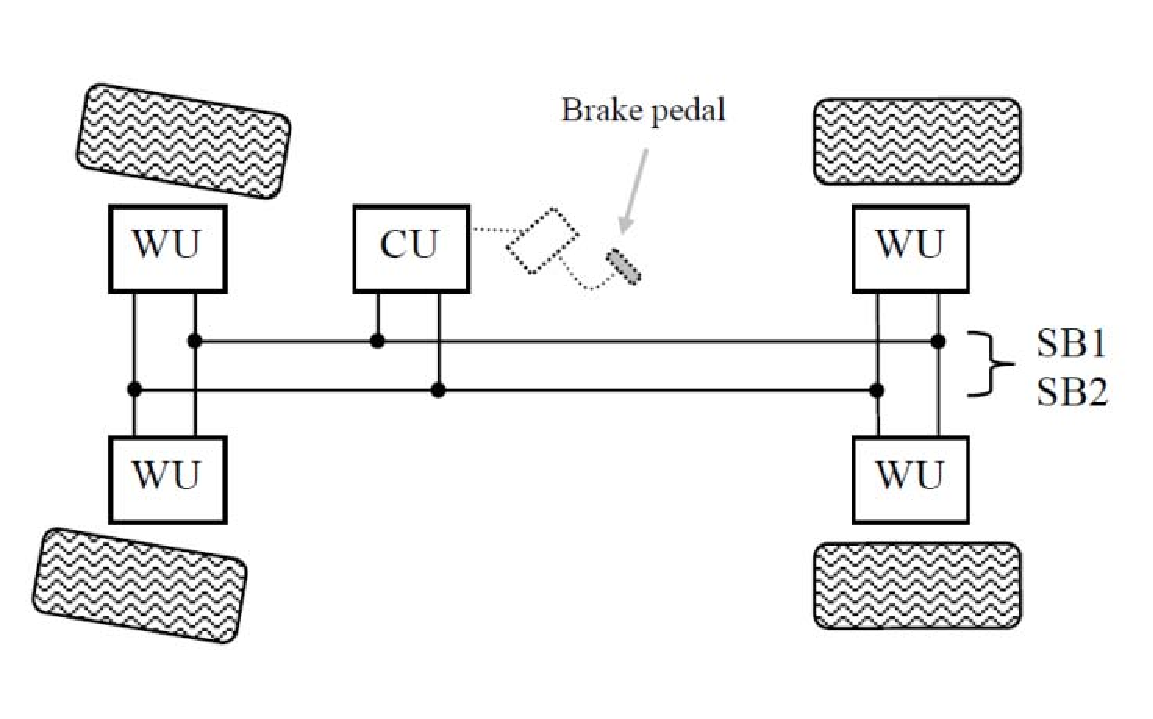
\includegraphics[scale=.5]{Fig1.pdf}
  \caption{Brake-by-wire system.}
  \label{bbwsys}
\end{figure}

%----------------------------------------------------------------------------------------
%	SECTION 2
%----------------------------------------------------------------------------------------
\newpage
\section{Overview of the Candidate Architecture}
\label{S2}
\todo[inline]{This section shall describe the centralized and distributed architectures, and the two modes of operation (full functionality and degraded functionality). It should also describe the modelling assumptions, including the model parameters.} 

%We will investigate two possible implementations of the system. In the first approach, the anti-lock control algorithms are executed locally in the wheel units. The complexity of the wheel units is in this design approximately the same as that of the central unit. However, the failure rate of the wheel units is higher than for the central unit, as they are more exposed to vibrations, moisture and temperature cycling. We call this design approach the distributed architecture. 

%The second approach is to execute the control algorithm for each wheel in the central unit, and let the wheel units consist of simple interfaces to the actuators and sensors. In this case, the control loops for anti-lock braking are closed over the communication network. The advantage with this approach is that the wheel units contain less hardware since they essentially consist of a communication interface, which sends data from the wheel speed sensor and receives commands to the brake actuator. Thus, the failure rate of the wheel units is lower compared to the other design. On the other hand, the failure rate of the central unit is higher, since it requires more processing power and more memory. We call this design approach the centralized architecture , since all control law calculations are performed by the central unit. 
\subsection{Centralized Architecture}
/text/
\subsection{Distributed Architecture}
\todo[inline]{Cite the reference list shall be formatted as the reference list in this document. For an example of how to write references, see Kopetz and Bauer [1]. (This paper is part of the course literature and is published by the Institute of Electrical and Electronics Engineers, Inc, known as IEEE, and therefore follows the IEEE format for scientific journal papers. Other publishers use slightly different formats.)\cite{lamport94}}
\subsection{Modes of Operation}
\todo[inline]{In this section you describe the two modes of operation of the system; full functionality and degraded functionality.}
\subsubsection{Full Functionality}
/text/
\subsubsection{Degraded Functionality}
/text/
\subsection{Assumptions and modeling parameters}
/text/
\begin{table}[h]
\centering
\begin{tabular}{| c | c | c | c |}
\hline 
Subsystem & Part & Failure rate & Coverage\\
\hline
System bus & Serial bus& FailureRate & 1\\
\hline
Wheel unit & Computer module & FailureRate & 1\\
\hline
Wheel unit & Sensor & FailureRate & 1\\
\hline
Wheel unit & Actuator & FailureRate & 1\\
\hline
Central unit & Computer module & FailureRate & 0.99\\
\hline
\end{tabular}
\caption{Failure rates and coverage factors for the distributed architecture}
\label{tab:Put a Lable}
\end{table}
\begin{table}[h]
\centering
\begin{tabular}{| c | c | c | c |}
\hline 
Subsystem & Part & Failure rate & Coverage\\
\hline
System bus & Serial bus& FailureRate & 1\\
\hline
Wheel unit & Computer module & FailureRate & 1\\
\hline
Wheel unit & Sensor & FailureRate & 1\\
\hline
Wheel unit & Actuator & FailureRate & 1\\
\hline
Central unit & Computer module & FailureRate & First CM failure:1 Second CM failure: 0.99\\
\hline
\end{tabular}
\caption{Failure rates and coverage factors for the Centralized Architecture}
\label{tab:Put a Lable}
\end{table}

\newpage
\section{Description of Models}
\label{S3}
In this section, models for the two architectures and their subsystems will be described.

\subsection{Wheel Unit Model}
Each wheel unit consists of three different components, sensors (S), actuator (A), and computing modules (CM), organized as in \figref{fig2}. There are two redundant CMs, two redundant sensors, and one actuator, yielding the reliability block diagram shown in \figref{fig3}.   
\begin{figure}[H]
  \centering
  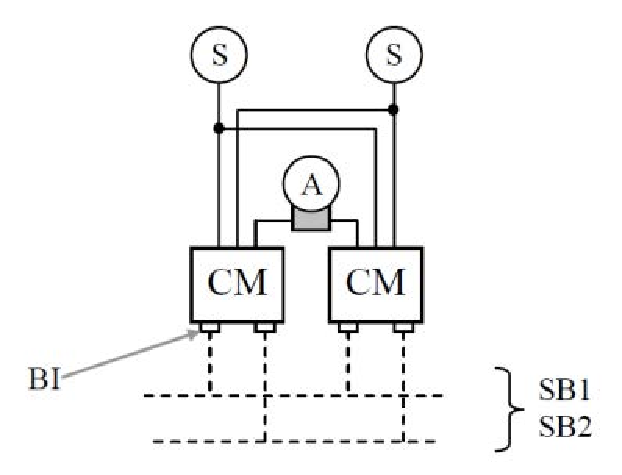
\includegraphics[scale=0.7]{Fig2.pdf}
  \caption{Wheel Unit}
  \label{fig2}
\end{figure}
\begin{figure}[H]
  \centering
  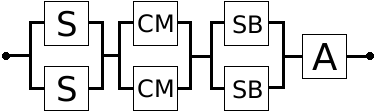
\includegraphics[scale=0.7]{wu_block.png}
  \caption{Reliability block diagram of the wheel unit}
  \label{fig3}
\end{figure}



%--------------------------------
\subsection{Wheel Unit Subsystem Model}
A combination of four WUs yields the wheel unit subsystem. In the full functionality mode of operation the subsystem can not tolerate any broken WUs, a fault tree in \figref{fig4} is shown for this mode. When running in the other mode of operation, allowing degraded functionality, one WU can become faulty without causing a full system failure, shown in \figref{fig5}. 
\begin{figure}[H]
  \Tree[.{WU Subsystem Failure} [.{$1 \geq$} WU WU WU WU ] ]
  \caption{Fault tree for the Wheel Unit Subsystem, full functionality}
  \label{fig4}
\end{figure}
\begin{figure}[H]
  \Tree[.{WU Subsystem Failure} [.{$2 \geq$} WU WU WU WU ] ]
  \caption{Fault tree for the Wheel Unit Subsystem, degraded functionality}
  \label{fig5}
\end{figure}


%--------------------------------
\subsection{Central Unit (CU)}
In the two evaluated architectures the central unit is configured in two different ways. The distributed architecture's central unit is described in \secref{subsec:dda} and the central unit for the centralized architecture is described in \secref{subsec:cta}. 

\subsubsection{Distributed Duplex Architecture}
\label{subsec:dda}
The distributed architecture's central unit consists of two computing modules (CM) configured in duplex. Each CM fails silent with a coverage factor of $99\%$. If a violation of the fail-silent property occurs, i.e. a CM delivers a erroneous result, the whole central unit fails. In \figref{fig6} the CMs and the serial buses (SB) connecting them, are illustrated. This setup yields the reliability block diagram shown in \figref{fig7}. As the subsystem works like a hot standby system with the failure rates and coverage factor from \tabref{tab:faildist}, the Markov chain model in \figref{fig8} can be derived.

\begin{figure}[H]
  \centering
  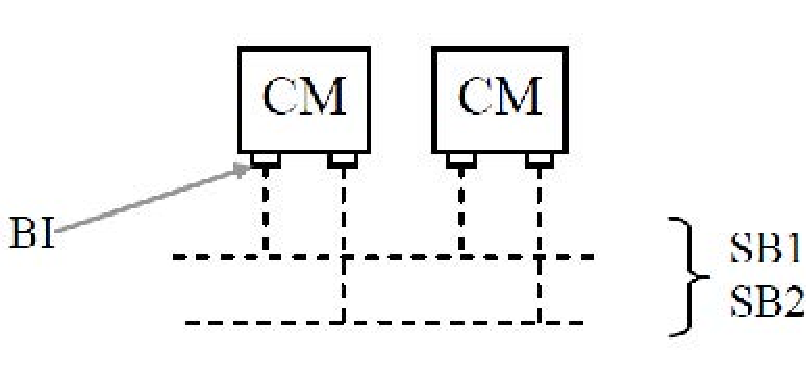
\includegraphics[scale=.5]{Fig6.pdf}
  \caption{Central Unit, duplex configuration }
  \label{fig6}
\end{figure}
\begin{figure}[H]
  \centering
  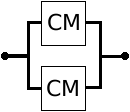
\includegraphics[scale=1.0]{cm2_block.png}
  \caption{Reliability block diagram for the Central Unit, duplex configuration}
  \label{fig7}
\end{figure}
\begin{figure}[H]
  \begin{center}
    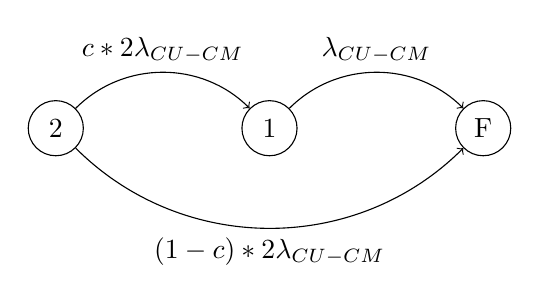
\begin{tikzpicture}[node distance=5mm and 20mm]
      \node[state] (s2) {2};
      \node[state] (s3) [right= of s2] {1};
      \node[state] (s4) [right= of s3] {F};
      \draw [->,bend left=45] (s2) to node[above] {$c*2\lambda_{CU-CM} $} (s3);
      \draw [->,bend right=45] (s2) to node[below] {$(1-c)*2\lambda_{CU-CM}$} (s4);
      \draw [->,bend left=45] (s3) to node[above] {$\lambda_{CU-CM}$} (s4);
    \end{tikzpicture}
  \caption{Markov chain model for central unit with duplex configuration}
   \label{fig8}
\end{center}
\end{figure}



%-------------
\subsubsection{Centralized Triplex Architecture}
\label{subsec:cta}
For the central unit in the centralized architecture, an additional CM is added making it a triplex configuration instead of duplex. When all three units is working the coverage factor for the first failure is 100\%. This as the three units produce results by majority voting, so even if one unit produces the wrong result, the voting masks it. A module producing an erroneous result is detected by the other modules and is shutdown. When this happens, the system reconfigures into a duplex system. 

How the CMs are connected can be seen in \figref{fig9}, and the corresponding reliability block diagram in \figref{fig10}. From the Markov chain model in \figref{fig11} it is easy to see that when the first unit fails, and a transition from state 3 to state 2 is made, the system behaves the same as the duplex configuration described in \secref{subsec:dda}. 

\begin{figure}[H]
  \centering
  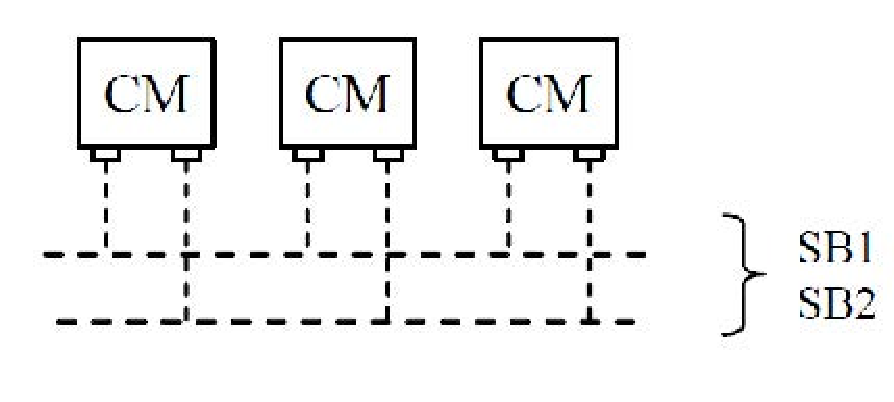
\includegraphics[scale=.5]{Fig9.pdf}
  \caption{Central Unit, triplex configuration }
  \label{fig9}
\end{figure}

\begin{figure}[H]
  \centering
  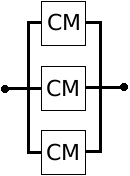
\includegraphics[scale=1.0]{cm3_block.png}
  \caption{Reliability block diagram for central unit in triplex configuration}
  \label{fig10}
\end{figure}
\begin{figure}[H]
  \centering
  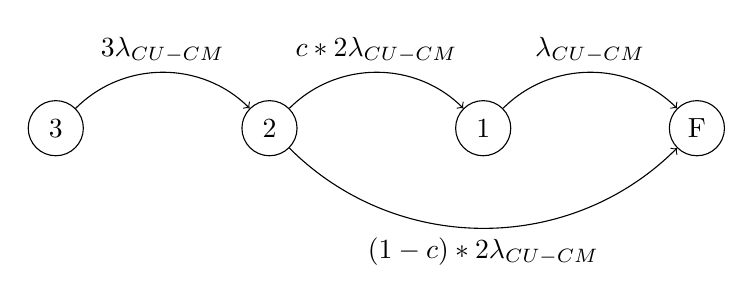
\begin{tikzpicture}[node distance=5mm and 20mm]
    \node[state] (sa) {3};
    \node[state] (sb) [right= of sa] {2};
    \node[state] (sc) [right= of sb] {1};
    \node[state] (sd) [right= of sc] {F};
    \draw [->,bend left=45] (sa) to node[above] {$3\lambda_{CU-CM} $} (sb);
    \draw [->,bend left=45] (sb) to node[above] {$c*2\lambda_{CU-CM} $} (sc);
    \draw [->,bend right=45] (sb) to node[below] {$(1-c)*2\lambda_{CU-CM}$} (sd);
    \draw [->,bend left=45] (sc) to node[above] {$\lambda_{CU-CM}$} (sd);
  \end{tikzpicture}
  \caption{Markov chain model for central unit in triplex configuration}
  \label{fig11}
\end{figure}





%--------------------------------
\subsection{System Model}
Here models for the two different system architectures and their modes of operation are described.

\subsubsection{Centralized Architecture}
\label{subsubsec:smca}
In \figref{fig12} a fault tree for the centralized architecture, running in the full functionality mode of operation, is displayed, and a fault tree for the degraded functionality is shown in \figref{fig13}. In both modes of operation it is clear from the fault trees that the system will still be working with two broken CMs and one broken SB, but for the degraded functionality mode of operation the system can handle one broken wheel unit, which the other mode can not.    

\begin{figure}[H]
  \Tree[.{System Failure} [.{$1 \geq$} [.{CU subsystem fail} [.{$\&$} CM CM CM ] ] [.{WU subsystem fail} [.{$1 \geq$} WU WU WU WU ] ] [.{SB subsystem fail} [.{\&} SB SB ] ] ] ]
  \caption{Fault tree for Full Functionality}
  \label{fig12}
\end{figure}
\begin{figure}[H]
  \Tree[.{System Failure} [.{$1 \geq$} [.{CU subsystem fail} [.{$\&$} CM CM CM ] ] [.{WU subsystem fail} [.{$2 \geq$} WU WU WU WU ] ] [.{SB subsystem fail} [.{\&} SB SB ] ] ] ]
  \caption{Fault tree for Degraded Functionality}
  \label{fig13}
\end{figure}

%-------------
\subsubsection{Distributed Architecture}
For the distributed architecture, fault trees for full functionality and degraded functionality is shown in \figref{fig14} and \figref{fig15}, respectively. The difference between them is the same as in \secref{subsubsec:smca}, with the exception that in this architecture, the system can only handle one broken CM before failing.

\begin{figure}[H]
  \Tree[.{System Failure} [.{$1 \geq$} [.{CU subsystem fail} [.{$\&$} CM CM ] ] [.{WU subsystem fail} [.{$1 \geq$} WU WU WU WU ] ] [.{SB subsystem fail} [.{\&} SB SB ] ] ] ]
  \caption{Fault tree for Full Functionality}
  \label{fig14}
\end{figure}
\begin{figure}[H]
  \Tree[.{System Failure} [.{$1 \geq$} [.{CU subsystem fail} [.{$\&$} CM CM ] ] [.{WU subsystem fail} [.{$2 \geq$} WU WU WU WU ] ] [.{SB subsystem fail} [.{\&} SB SB ] ] ] ]
  \caption{Fault tree for Degraded Functionality}
  \label{fig15}
\end{figure}
\newpage
\section{Results}
/{Describe the results. Graphs and tables shall be commented in text. To facilitate the comparison of the results for different design solutions, include several reliability graphs in one diagram.}/
\begin{table}[h]
\centering
\begin{tabular}{| c | c | c | c |}
\hline
\multicolumn{2}{|c|}{Units} & Distributed & Centralized\\
\hline
\multirow{2}{*}{Wheel Unit Subsystem Full Functionality} & Reliability & 0.7450 & 0.8357\\
 & MTTF & 3.93  & 5.52\\
\hline
\multirow{2}{*}{Wheel Unit Subsystem Degraded Functionality}& Reliability & 0.9726  & 0.9891\\
 & MTTF & 7.24 & 10.2\\
\hline
\multirow{2}{*}{Central Unit}& Reliability& 0.9806  & 0.9952\\
 & MTTF & 21.3  & 20.8\\
\hline
\multirow{2}{*}{Entire System Full Functionality}& Reliability & 0.7305  & 0.8316\\
 & MTTF & 3.74 & 5.23\\
\hline
\multirow{2}{*}{Entire System Degraded Functionality}& Reliability & 0.9537 & 0.9843\\
 & MTTF & 6.56 & 9.06\\
\hline
\end{tabular}
\caption{Reliability and MTTF results}
\label{tab:Put a Lable}
\end{table}
\\/{Insert Reliability Graphs and comment them in the text. Make sure that the caption numbers are correct.}/
\newpage
\section{Discussion}
\label{S5}
/{Discuss the pros and cons of the different design solutions.} /

\newpage
\section{Conclusions}
\label{S6}
/{Present your conclusions and recommendations.}/\cite{sharpe}\cite{gnuplot}

The choice of implementing either of the two designs is influenced by more factors than the results of a reliability evaluation as conducted in this laboratory assignment. Other properties that is of value is for example cost, maintainability, and modifiability. The cost is of coarse of major concern and the maintenance can be a significant part of the life-time cost. It is hard for us to guess about any cost differences, as the two systems utilize the same amount of hardware. One point in favor for the centralized architecture is that it is probably easier to physically replace a computer module in the CU than in a WU. If the software is updated with more complex routines, the CMs which derives the brake commands must maybe be upgraded. In the centralized design three CMs need to be replaced, compared to eight in the distributed design. However, the CMs replaced in the centralized design has higher processing capabilities but are, as mentioned, probably easier to replace, the lesser time it takes to replace the three MCs versus the eight makes it probably more cost effective to use the centralized design. 
\addcontentsline{toc}{section}{References}

\begin{thebibliography}{9}
\bibitem{lamport94}
  Leslie Lamport,
  \emph{\LaTeX: A Document Preparation System}.
  Addison Wesley, Massachusetts,
  2nd Edition,
  1994.

Please use Vancouver/IEEE style for your referencing. For more information please check: http://www.lib.unimelb.edu.au/cite/ieee/index.html
\\
The reference list shall be formatted as the reference list in this document. For an example of how to write references, see Kopetz and Bauer [1]. (This paper is part of the course literature and is published by the Institute of Electrical and Electronics Engineers, Inc, known as IEEE, and therefore follows the IEEE format for scientific journal papers. Other publishers use slightly different formats.)

\end{thebibliography}


\end{document}
